\section{Visão Geral}

A figura~\ref{fig:pus_overview} apresenta a visão geral da comunicação solo-bordo do ponto de vista de serviços do PUS (\textit{Packet Utilization Standard}), como descrito em [DR2].

\begin{figure}[H]
    \centering
    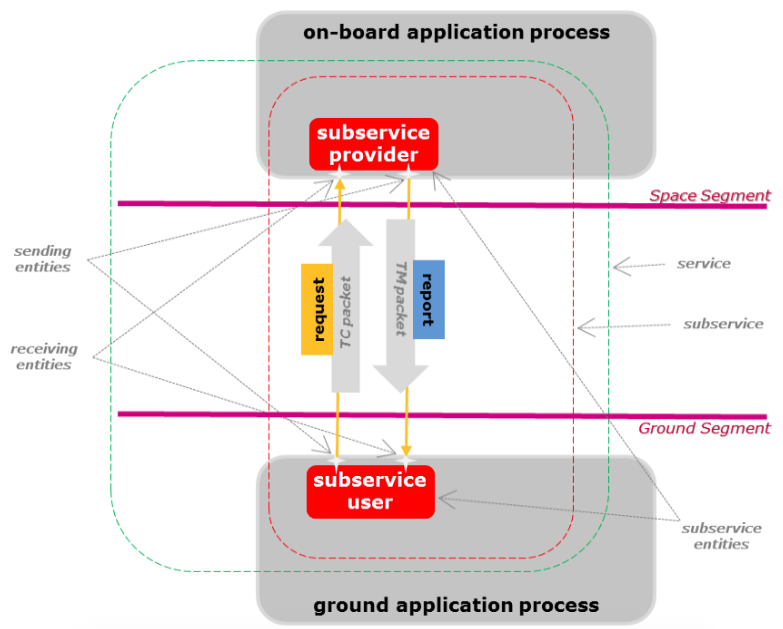
\includegraphics[width=0.6\textwidth]{pus_context.png}
    \caption{Visão geral do contexto solo-bordo por serviço do PUS [DR2].}
    \label{fig:pus_overview}
\end{figure}

A divisão entre segmento espacial e segmento solo se dá, além de fisicamente, de forma quanto às funções exercidas.
Todos os processos ativos à bordo da plataforma são classificados como provedores de subserviços e as aplicações em solo, os usuários destes.
Assim, a mesuração de uma plataforma espacial se dá pela prestação dos serviços as quais ela é capaz de prover.

A informação trocada entre os usuários e provedores de cada subserviço é chamada de "\textbf{mensagem}".
Uma mensagem é transmitida semanticamente intocada através do protocolo de comunicação que conecta usuários e provedores, ou seja solo-bordo.

Uma mensagem transmitida de um usuário a um provedor de dado subserviço, a fim de invocar a execução de atividades à bordo, é chamado de ``\textbf{requisição}".
Cada requisição pode conter uma ou mais instruções, telecomandos.
Uma mensagem enviada por um provedor a um usuário de dado subserviço é chamado de ``\textbf{relatório}".
Cada relatório contém uma ou mais notificações, telemetrias.

Existem três tipos de categorias de relatório:

\begin{enumerate}[label=\roman*.]
    \item \textit{relatórios de verificação}, cada relato de roteamento, confirmação, início, progresso e término da execução de uma requisição, e.g. \textit{ping} em um subsistema específico;
    \item \textit{relatórios de dados}, que são gerados:
    \begin{enumerate}[label=(\alph*)]
        \item sob requisição, uma ou múltiplas respostas às instruções em uma requisição com algum tipo de dado de um determinado serviço, e.g. dados de missão,
        \item relatório gerados de forma automática por requisição ou, rotineiramente, e.g. \textit{beacon};
    \end{enumerate}
    \item \textit{relatórios de eventos}, traz informações relacionadas a ocorrências de eventos detectados por um serviço, \textit{log} de eventos.
\end{enumerate}

\subsection{Entidades e Interfaces}

A figura~\ref{fig:interfaces} apresenta a principais entidades evolvidas e interfaces na comunicação solo-bordo.

\begin{figure}[H]
    \centering
    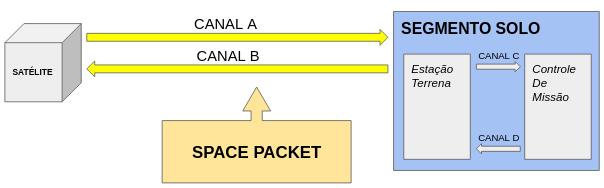
\includegraphics[width=0.65\textwidth]{figures/cubed_interfaces.png}
    \caption{Entidades e Interfaces para a Comunicação Solo-Bordo}
    \label{fig:interfaces}
\end{figure}

Duas entidades são descritas, o segmento espacial, i.e. satélite, e o segmento solo.
As mensagens trocadas entre o segmento solo e o satélite é, a partir de agora, chamado de "\textbf{Space Packet}".

O \textit{Space Packet} é transmitido em dois canais distintos, Canal A e Canal B, \textit{downlink} e \textit{uplink}, respectivamente.
Suas interfaces com o satélite são representadas pelo subsistema de Rastreio, Telemetria e Comando (TT\&C) e com o Segmento Solo, pela Estação Terrena.

A seguir, temos três requisitos principais que o satélite deve atender.

\begin{table}[H]
    \centering
    \begin{tabular}{|c|c|}
        \hline
        \rowcolor{orange}
        \textbf{RQ-SYS-211} & \textbf{O satélite deve se comunicar com o segmento solo via \textit{space packets}} \\ \hline
    \end{tabular}
    \label{tab:rq-sys-101}
\end{table}

\begin{table}[H]
    \centering
    \begin{tabular}{|c|c|}
        \hline
        \rowcolor{orange}
        \textbf{RQ-SYS-212} & \textbf{O satélite deve enviar telemetrias ao segmento solo via canal A.} \\ \hline
    \end{tabular}
    \label{tab:rq-sys-102}
\end{table}

\begin{table}[H]
    \centering
    \begin{tabular}{|c|c|}
        \hline
        \rowcolor{orange}
        \textbf{RQ-SYS-213} & \textbf{O satélite deve receber comandos do segmento solo via canal B.} \\ \hline
    \end{tabular}
    \label{tab:rq-sys-103}
\end{table}

\subsection{Segmento Solo}

O segmento solo consta de duas entidades, \textit{Estação Terrena} e \textit{Controle de Missão} [DR1].

\subsubsection{Estação Terrena}

A estação terrena busca realizar a interface entre o segmento espacial e o segmento solo, mais precisamente o controle da missão.

A estação terrena tem, por objetivo, (i) receber o \textit{space packet}, realizar as adequações necessárias ao sinal recebido e disponibilizar a telemetria a ser decodificada pelo Controle de Missão e, (ii) receber o \textit{space packet}, realizar as adequações necessárias ao sinal, em radio-frequência, a ser transmitido para o segmento espacial.

\subsubsection{Controle de Missão}

O Controle de Missão é o ponto de convergência da operação da missão.
Sendo capaz de decodificar os \textit{space packets} de telemetria e codificar os \textit{space packets} de telecomandos.

\subsection{Canais de Interface}

\subsubsection{Canal A}

O Canal A é a representação do canal de \textit{downlink} de relatórios do satélite.
Por este canal serão transmitidos os relatórios (telemetrias) e dados (dados de missão), verificação (beacon) e log de eventos do satélite.

Visto que o desafio do subsistema de TT\&C não se aterá às características de radio-frequência, as mensagens transmitidas no canal A devem ser apenas moduladas, digitalmente.

Entre os métodos de modulação digital, será utilizado a modulação \textbf{BPSK} -- \textit{Binary Phase Shifting Keying}, vide Apêndice~\ref{sec:bpsk}.

\begin{table}[H]
    \centering
    \begin{tabular}{|c|c|}
        \hline
        \rowcolor{orange}
        \textbf{RQ-TTC-231} & \textbf{O canal de \textit{downlink} deve ser modulado em BPSK.} \\ \hline
    \end{tabular}
    \label{tab:rq-ttc-011}
\end{table}

\subsubsection{Canal B}

O Canal B é a representação do canal de \textit{uplink} de requisições do satélite.
Por este canal serão transmitidas as requisições (telecomandos) de serviços e subserviços de usuários a partir do segmento solo.

Visto que o desafio do subsistema de TT\&C não se aterá às características de radio-frequência, as mensagens transmitidas no canal A devem ser apenas moduladas, digitalmente.

Entre os métodos de modulação digital, será utilizado a modulação \textbf{BPSK} -- \textit{Binary Phase Shifting Keying}, vide Apêndice~\ref{sec:bpsk}.

\begin{table}[H]
    \centering
    \begin{tabular}{|c|c|}
        \hline
        \rowcolor{orange}
        \textbf{RQ-TTC-232} & \textbf{O canal de \textit{uplink} deve ser demodulado em BPSK.} \\ \hline
    \end{tabular}
    \label{tab:rq-ttc-021}
\end{table}

\subsubsection{Canal C}

O Canal C é a representação do canal comunicação entre a Estação Terrena e o Controle de Missão, no qual são recebidas as telemetrias as serem decodificadas.

\subsubsection{Canal D}

O Canal D é a representação do canal comunicação entre o Controle de Missão e a Estação Terrena, no qual são transferidos os comandos a serem enviados ao segmento espacial.